\subsection*{Technical Performance Mesurement}
\begin{frame}{Technical Performance Mesurement}
    \begin{itemize}
        \item Classification Accuracy
        \item Latency
        \item Robustness
        \item Other Metrics
    \end{itemize}
\end{frame}

\begin{frame}{TPM \textemdash{} Classification Accuracy}

\begin{table}[!htbp]
    \centering
    \begin{tabular}{|c||c|c|c|c|}
        \hline
        & \textbf{Feet} & \textbf{Left Hand} & \textbf{Right Hand} & \textbf{Rest} \\
        \hline
        \hline
        \textbf{Feet} & \textbf{779} & 367 & 259 & 314 \\
        \hline
        \textbf{Left Hand} & 284 & \textbf{1005} & 189 & 258 \\
        \hline
        \textbf{Right Hand} & 356 & 243 & \textbf{840} & 268 \\
        \hline
        \textbf{Rest} & 1474 & 1188 & 1158 & \textbf{3067} \\
        \hline
    \end{tabular}
    \caption{Confusion matrix of the validation dataset. \textbf{47.23\%} Accuracy}
\end{table}
\begin{table}[!htbp]
    \centering
    \begin{tabular}{|c||c|c|c|c|}
        \hline
        & \textbf{Feet} & \textbf{Left Hand} & \textbf{Right Hand} & \textbf{Rest} \\
        \hline
        \hline
        \textbf{Feet} & \textbf{824} & 104 & 38 & 34 \\
        \hline
        \textbf{Left Hand} & 16 & \textbf{961} & 1 & 22 \\
        \hline
        \textbf{Right Hand} & 28 & 51 & \textbf{789} & 132 \\
        \hline
        \textbf{Rest} & 1 & 6 & 1 & \textbf{992} \\
        \hline
    \end{tabular}
    \caption{Confusion matrix of the GAN data. \textbf{89.15\%} Accuracy}
\end{table}

\end{frame}
\begin{frame}{TPM \textemdash{} Latency}
    \begin{figure}[!htbp]
        \scalebox{1}[1]{
        \begin{tikzpicture}
            % Horizontal line
            \draw[thick] (0,0) -- (7.6625,0);
            \draw[thick, dashed] (7.6625,0) -- (8.15,0);
            \draw[thick, -Triangle] (8.15,0) -- (10,0) node[font=\scriptsize,below left=3pt and -8pt]{\textbf{ms}};
            % \draw[thick, dashed] (9,0) -- (9.5,0);
            % \draw[thick, -Triangle] (9,0) -- (10,0) node[font=\scriptsize,below left=3pt and -8pt]{\textbf{ms}};
    
            % Start of the timeline
            \draw (0,-0.1) -- (0,0.1) node[font=\scriptsize,below left=3pt and -6pt]{\textbf{0}};
            \node[font=\scriptsize,left=3pt] at (0,0) [anchor=east]{\textbf{Min}};
    
            % Image Processing Time
            \draw (0.1625, -0.1) -- (0.1625, 0.1) node[font=\scriptsize,below left=3pt and -10pt]{\textbf{\textcolor{olive}{13}}};
            \fill[purple] (0, 0.2) rectangle (0.1625, 0.4);
            
            % \draw (1, -0.1) -- (1, 0.1) node[font=\scriptsize,below left=3pt and -8pt]{\textbf{\textcolor{red}{80}}};
            % \fill[purple] (0,-0.4) rectangle (1,-0.6);
            
            % Motor Response Time
            \draw (1.4125, -0.1) -- (1.4125, 0.1) node[font=\scriptsize,below left=3pt and -10pt]{\textbf{\textcolor{olive}{113}}};
            \fill[blue] (0.1625, 0.4) rectangle (1.4125, 0.6);
    
            % \draw (2.75, -0.1) -- (2.75, 0.1) node[font=\scriptsize,below left=3pt and -10pt]{\textbf{\textcolor{red}{220}}};
            % \fill[blue] (1,-0.6) rectangle (2.75,-0.8);
    
            % Motor Response Recording Time
            \draw (7.6625, -0.1) -- (7.6625, 0.1) node[font=\scriptsize,below left=3pt and -8pt]{\textbf{\textcolor{olive}{613}}};
            \fill[red] (1.4125, 0.6) rectangle (7.6625, 0.8);
    
            % \draw (9, -0.1) -- (9, 0.1) node[font=\scriptsize,below left=3pt and -10pt]{\textbf{\textcolor{red}{720}}};
            % \fill[red] (2.75,-0.8) rectangle (9,-1);
    
            % Signal Classification Time
            \draw (8.15, -0.1) -- (8.15, 0.1) node[font=\scriptsize,below left=3pt and -10pt]{\textbf{\textcolor{olive}{615}}};
            \fill[amethyst] (7.6625, 0.8) rectangle (8.15, 1);
    
            % \draw (9.5, -0.1) -- (9.5, 0.1) node[font=\scriptsize,below left=3pt and -10pt]{\textbf{\textcolor{red}{732}}};
            % \fill[amethyst] (9,-1) rectangle (9.5,-1.2);
    
            % diff curly brace
            % \draw [decorate,decoration={brace,amplitude=5pt}] (8.15, 1) -- (9.5,1) node [anchor=south,midway,above=4pt] {\footnotesize Signal Received by Application};
        \end{tikzpicture}
        }
        \scalebox{1}[1]{
        \begin{tikzpicture}
                % Horizontal line
                \draw[thick] (0,0) -- (9,0);
                % \draw[thick, dashed] (7.6625,0) -- (8.15,0);
                % \draw[thick] (8.15,0) -- (9,0);
                \draw[thick, dashed] (9,0) -- (9.5,0);
                \draw[thick, -Triangle] (9.5,0) -- (10,0) node[font=\scriptsize,below left=3pt and -8pt]{\textbf{ms}};
    
                % Start of the timeline
                \draw (0,-0.1) -- (0,0.1) node[font=\scriptsize,below left=3pt and -6pt]{\textbf{0}};
                \node[font=\scriptsize,left=3pt] at (0,0) [anchor=east]{\textbf{Max}};
    
                % Image Processing Time
                % \draw (0.1625, -0.1) -- (0.1625, 0.1) node[font=\scriptsize,below left=3pt and -10pt]{\textbf{\textcolor{olive}{13}}};
                % \fill[purple] (0, 0.2) rectangle (0.1625, 0.4);
                
                \draw (1, -0.1) -- (1, 0.1) node[font=\scriptsize,below left=3pt and -8pt]{\textbf{\textcolor{red}{80}}};
                \fill[purple] (0,0.2) rectangle (1,0.4);
                
                % Motor Response Time
                % \draw (1.4125, -0.1) -- (1.4125, 0.1) node[font=\scriptsize,below left=3pt and -10pt]{\textbf{\textcolor{olive}{113}}};
                % \fill[blue] (0.1625, 0.4) rectangle (1.4125, 0.6);
    
                \draw (2.75, -0.1) -- (2.75, 0.1) node[font=\scriptsize,below left=3pt and -10pt]{\textbf{\textcolor{red}{220}}};
                \fill[blue] (1,0.4) rectangle (2.75,0.6);
    
                % Motor Response Recording Time
                % \draw (7.6625, -0.1) -- (7.6625, 0.1) node[font=\scriptsize,below left=3pt and -8pt]{\textbf{\textcolor{olive}{613}}};
                % \fill[red] (1.4125, 0.6) rectangle (7.6625, 0.8);
    
                \draw (9, -0.1) -- (9, 0.1) node[font=\scriptsize,below left=3pt and -10pt]{\textbf{\textcolor{red}{720}}};
                \fill[red] (2.75,0.6) rectangle (9,0.8);
    
                % Signal Classification Time
                % \draw (8.15, -0.1) -- (8.15, 0.1) node[font=\scriptsize,below left=3pt and -10pt]{\textbf{\textcolor{olive}{614}}};
                % \fill[amethyst] (7.6625, 0.8) rectangle (8.15, 1);
    
                \draw (9.5, -0.1) -- (9.5, 0.1) node[font=\scriptsize,below left=3pt and -10pt]{\textbf{\textcolor{red}{745}}};
                \fill[amethyst] (9,0.8) rectangle (9.5,1);
    
                % diff curly brace
                % \draw [decorate,decoration={brace,amplitude=5pt}] (8.15, 1) -- (9.5,1) node [anchor=south,midway,above=4pt] {\footnotesize Signal Received by Application};    
        \end{tikzpicture}
        }
        \begin{itemize}
            \item \textcolor{purple}{Brain Processing Image Time:} 13-80 ms
            \item \textcolor{blue}{Brain Motor Response Activation Time:} 100-140 ms
            \item \textcolor{red}{BCI Motor Response Recording Time:} 500 ms
            \item \textcolor{amethyst}{Signal Classification Time:} 1.10-24.67 ms
        \end{itemize}
        \caption{Latency of the system in a real case scenario.}\label{fig:latency}
    \end{figure}
\end{frame}
\begin{frame}{TPM \textemdash{} Robustness}
    \begin{figure}[!htbp]
        \centering
        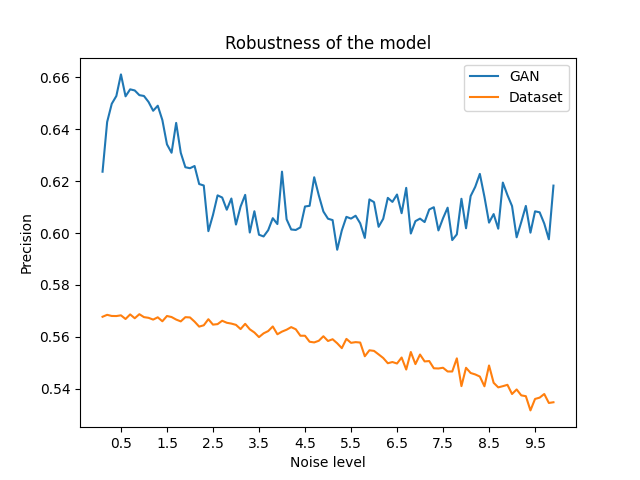
\includegraphics[width=0.8\textwidth]{figures/Testing/robustness_plot}
        \caption{Robustness of the system in case of noise in the data.}\label{fig:robustness}
    \end{figure}
\end{frame}
\begin{frame}{TPM \textemdash{} Other Metrics}
    \begin{itemize}
        \item Portability: Written in Python with Torch for CUDA
        \item Efficiency: Can run on most modern Hardware Platforms
        \item Maintainability: 6.55 PyLint Score
    \end{itemize}
    \begin{table}[!htbp]
        \centering
        \scalebox{.8}{
        \begin{tabular}{|c||c|c|c|}
            \hline
            \textbf{Resource} & \textbf{Minimum Usage} & \textbf{Average Usage} & \textbf{Maximum Usage} \\
            \hline
            \hline
            K-FLOPS & 754 & 754 & 754\\
            \hline
            CPU Memory & 30 KB & 47 KB & 90 KB \\
            \hline
            GPU CUDA Memory & 277 KB & 17.7 MB  & 41.3 MB \\
            \hline
        \end{tabular}
        }
        \caption{Efficiency of the system in terms of resource usage.}
    \end{table}
\end{frame}
